\appendix

\section{The decoding pipeline}
\label{app:pipeline}

Figure~\ref{fig:pipeline} places the repair layer in the loop it runs inside.
Every denoising step advances the parser over whatever prefix has become
contiguous; a rejection routes through a termination test and a bounded
single-token retry before the joint search is invoked, and every outcome except
emission returns to the next step. The shaded box is the contribution of this
paper; the rest is the frontier-constrained decoder it sits on.

\begin{figure}[h]
\centering
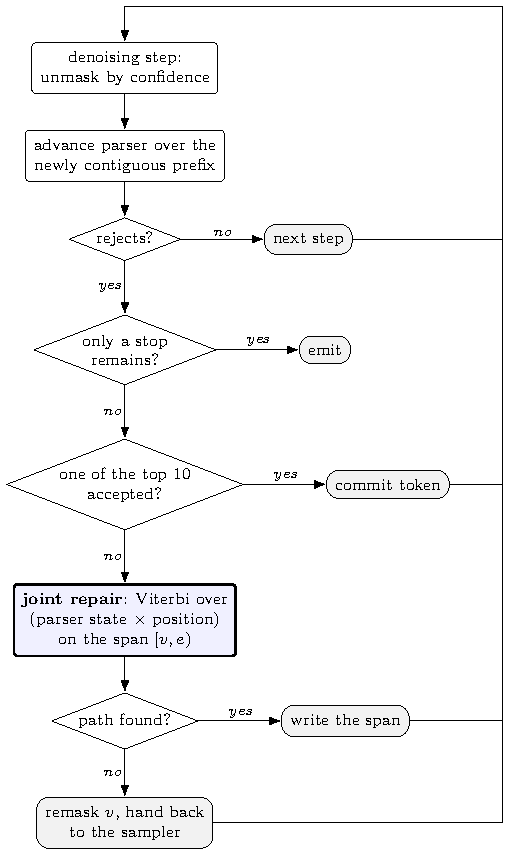
\includegraphics[width=0.52\linewidth]{pipeline.pdf}
\caption{Where the joint repair fires. Only a parser rejection reaches it, and
only after a stop test and a bounded retry have failed, so a clean step pays
nothing.}
\label{fig:pipeline}
\end{figure}

\section{The distribution of legal token sets}
\label{app:legalsets}

Section~\ref{sec:cand} rests on a claim about how many tokens an incremental
parser actually admits at a live state. This appendix gives the measurement and
the full distribution.

\paragraph{Procedure.}
We take the $40$ generated outputs of the DPGrammar run on JSONSchemaBench
\texttt{medium} (seed $0$, $T{=}128$) whose schemas compile, and replay each one
through \texttt{llguidance}~1.7.0 under teacher forcing: the parser is
initialised from the instance's schema, and the tokens the model actually
produced are fed to it one at a time. Before consuming each token we call
\texttt{compute\_logit\_bias()} and count the non-zero entries of the returned
mask; that count is $|\mathcal{L}(q)|$, the number of tokens the parser would
accept next. Replay stops at the first token the parser rejects, so every state
we record is one the decoder genuinely reached. This yields $6{,}657$ live
states over a vocabulary of $|V|=126{,}349$. The measurement is offline and
model-free, which needs only the schema and the emitted text, so it can be
reproduced without a GPU.

\paragraph{The distribution.}
Figure~\ref{fig:legalsets} shows the result. The distribution is not merely
skewed, it is bimodal: $38.4\%$ of states admit fewer than $100$ tokens
and $29.7\%$ admit more than $10{,}000$, leaving the decade between $10^4$ and
$10^5$ nearly empty. The median is $106$. The extremes are sharper still: before the first token
a JSON object grammar admits $2$ of $126{,}349$ tokens, and after the two
characters \texttt{\{\char34} it admits exactly one, the first character of
the only property name the schema allows there.

\begin{figure}[h]
\centering
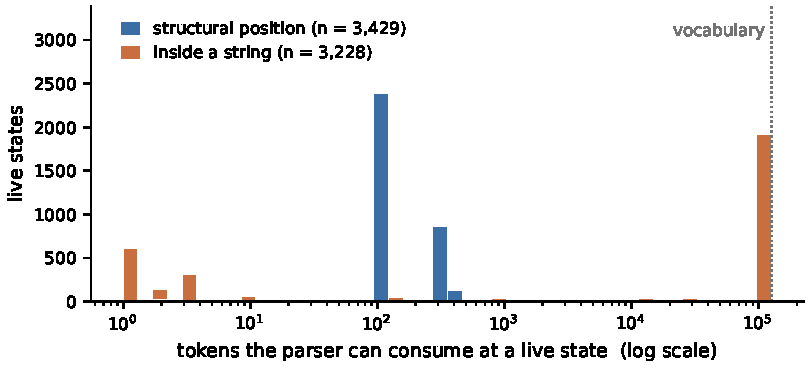
\includegraphics[width=0.86\linewidth]{legal_sets.pdf}
\caption{How many tokens an incremental parser admits, over $6{,}657$ live
states on JSONSchemaBench \texttt{medium} ($|V|=126{,}349$). The distribution is
bimodal and the decade between the modes is nearly empty, which is why no single
$k$ suits both. Structural positions are uniformly tight; the bimodality lives
inside strings, separating a partially spelled property name, which admits a
handful of continuations, from a free-form value, which admits almost the whole
vocabulary.}
\label{fig:legalsets}
\end{figure}

\paragraph{What the order of proposal and filter costs.}
The distribution above is why \S\ref{sec:cand} draws candidates from
$\mathcal{L}(q)$ rather than ranking $V$ and filtering. On \texttt{medium} the
admitted set is smaller than a top-$100$ draw at $38\%$ of live states, so a
filter-then-propose scheme is sampling against a small target at those
positions; conversely the set is smaller than $k$ at $40\%$ of state-positions,
where the edge set is enumerated exactly rather than sampled and the search at
that node is exhaustive rather than heuristic. Reversing the order in our own
implementation costs $1.2$\,pp of schema@1 and produces four repair sites where
the draw contained no token the parser would accept, a class the edge set cannot
produce (\S\ref{sec:ablation}).

\paragraph{Where the two modes come from.}
The obvious explanation, that the tight mode is structural punctuation and the
wide mode is string content, is only half right. Structural positions
($3{,}429$ states) are uniformly tight, with a median of $104$ and a quartile
range of $95$ to $324$. The bimodality lives entirely inside strings ($3{,}228$
states, p25 $=3$, median $=125{,}308$), where it separates two kinds of string:
a free-form value admits almost the whole vocabulary, whereas a partially
spelled property name admits a handful of continuations. Both modes matter for
repair. The wide one is where filtering a top-$k$ draw is wasteful but harmless;
the tight one is where it fails, and the tight one contains exactly the
positions a diffusion decoder is most likely to get wrong: key boundaries,
closings, and enumerated values.

\paragraph{When the automaton gives the complete candidate set.}
Where $|\mathcal{L}(q)| \le k$, Eq.~\ref{eq:cand} enumerates the edge set exactly rather
than sampling it, and the candidate set is provably complete:

\begin{center}
\small
\begin{tabular}{lrrrrrr}
\toprule
$k$ & $8$ & $32$ & $64$ & $100$ & $128$ & $256$ \\
\midrule
states with $|\mathcal{L}(q)| \le k$ & $16.4\%$ & $17.9\%$ & $18.1\%$ & $39.7\%$ & $54.0\%$ & $54.6\%$ \\
\bottomrule
\end{tabular}
\end{center}

The jump between $k{=}64$ and $k{=}128$ is the tight mode itself, which clusters
near $100$; this is why we set $k=100$ and why raising it further buys little.
The fraction varies widely across schemas (at $k{=}32$: median $18.4\%$,
interquartile range $9.8$--$28.3\%$, and $100\%$ for the most constrained schema
in the sample), so it is a property of the schema, not a constant of the
tokenizer.

\paragraph{Two facts the method depends on.}
First, no live state had an empty legal set ($0$ of $6{,}657$). This is what
makes the DP total: a live state always has a continuation, so the candidate set
is never empty and the search can always complete the span. Our termination rule
(\S\ref{sec:stop}) treats an empty mask as a failed read rather than as a stop
signal for this reason. Second, the mask read is cheap ($0.025$\,ms mean,
$0.012$\,ms median) and the implementation already performs it to compute the
state key used for path merging, so drawing candidates from the automaton adds
no parser calls beyond those already paid for.



\section{Ordering artifacts}
\label{app:ordering}

llguidance compiles a JSON schema into a grammar that fixes the order of an
object's properties to their declaration order: \texttt{\{"a":1,"b":2\}} is
rejected when the schema declares \texttt{b} first, although both orders satisfy
the schema and \texttt{jsonschema} accepts either. A model that writes the
properties in a different order therefore produces a violation that is not an
error, and the correct repair, moving a block, is not expressible by a
positional DP, which can only overwrite in place. The repair then writes the
demanded key name over a value intended for another field. We measured this class
at $7.6\%$ of $118$ violations; among the $16$ that occur where the grammar
admits exactly one token, half are of this kind.


\section{The parser interface}
\label{app:api}

The paper treats the incremental parser abstractly: a state $q$, a consumable
set $\mathcal{L}(q)$, and the ability to advance, copy, and undo. This appendix
records the concrete interface those abstractions are built on, so that the
method can be reimplemented against a different parser.

\paragraph{Construction.}
We use \textsc{llguidance}~1.7.0 \citep{microsoft2025llguidance}. A tokenizer is
built from the checkpoint's own \texttt{tokenizer.json}, so token boundaries in
the grammar and in the model agree exactly. A JSON Schema is compiled with
\texttt{grammar\_from\_json\_schema} and a SMILES grammar with
\texttt{grammar\_from\_lark}; compilation is checked before use, and a schema
that fails to compile is excluded from every arm rather than scored as a failure
for one (Table~\ref{tab:coverage} quantifies how many). We raise the default parser
limits to \texttt{max\_items\_in\_row}${=}20{,}000$ and
\texttt{step\_max\_items}${=}600{,}000$; at the defaults, deeply nested schemas
abort mid-parse.

\paragraph{The five operations.}
\begin{center}
\small
\begin{tabular}{lll}
\toprule
paper & \textsc{llguidance} & note \\
\midrule
$\mathcal{L}(q)$        & \texttt{compute\_logit\_bias()}    & byte mask over $V$; $0.025$\,ms mean \\
advance                 & \texttt{try\_consume\_tokens([t])} & returns tokens consumed; $0$ means rejected \\
copy a state            & \texttt{deep\_copy()}              & lattice nodes hold these \\
undo                    & \texttt{rollback(n)}               & probe without copying \\
may stop                & \texttt{is\_accepting()}           & state is final, not that it must stop \\
\bottomrule
\end{tabular}
\end{center}

\paragraph{Two details the method depends on.}
First, \textsc{eos} is marked legal by the bias at accepting states but is not a
consumable grammar symbol: \texttt{try\_consume\_tokens([\textsc{eos}])} returns
$0$ there. It is therefore excluded from the candidate set of
Eq.~\ref{eq:cand}: offering it wastes a slot, and where it is the only token the
bias marks legal it would empty the set and imitate a dead end. A termination rule written in terms of consumption would therefore
never fire, which is why \texttt{only\_stop\_remains} (\S\ref{sec:stop}) is
defined on the bias---nothing but stop tokens remains legal---rather than on
what the parser will consume. Second, the DP merges lattice paths on
\texttt{bytes}(\texttt{compute\_logit\_bias()}) as the state key: two parser
states that admit exactly the same tokens are indistinguishable to every
subsequent decision, so collapsing them is exact rather than an approximation.
The key is a value the implementation already computes to build the candidate
set, so merging costs no additional parser calls.




\section{Grammar coverage and the CD-CFG comparison}
\label{sec:coverage}

\begin{table}[t]
\centering
\small
\caption{Grammar coverage is a property of the compiler, not of the decoder.
Each arm inherits the schemas its toolchain accepts; validity is then measured
only on the $351$ \texttt{medium} schemas both toolchains compile, so the two
effects are not confounded.}
\label{tab:coverage}
\begin{tabular}{llcc}
\toprule
Method & Toolchain & Schemas compiled & Validity on the shared $351$ \\
\midrule
CD-CFG             & \textsc{rustformlang} & $383/586$ ($65.4\%$) & $45.0\%$ \\
LAVE               & \textsc{llguidance}   & $511/586$ ($87.2\%$) & $82.3\%$ \\
No-DP baseline     & \textsc{llguidance}   & $511/586$ ($87.2\%$) & $92.6\%$ \\
\textbf{DPGrammar} & \textsc{llguidance}   & $511/586$ ($87.2\%$) & $\mathbf{97.4\%}$ \\
\bottomrule
\end{tabular}
\end{table}

CD-CFG~\citep{cd4dllm} is run from the authors' released code, which builds its
constraint with \textsc{rustformlang}, the formal-language library distributed
in the same repository, rather than with
\textsc{llguidance}~\citep{microsoft2025llguidance}. The two
accept different schemas: $351$ compile under both, $160$ only under
\textsc{llguidance}, $32$ only under \textsc{rustformlang}, with
\textsc{rustformlang} rejecting $203$ of $586$ mostly over regular-expression
quantifiers that Python's \texttt{re} accepts.

Counting those $203$ as decoding failures would measure a regex front-end
rather than a decoding algorithm, so we report coverage separately and compare
decoding only on the shared $351$. There CD-CFG reaches $45.0\%$ validity with
$19$ timeouts against DPGrammar's $97.4\%$ with none, and the ordering of the
arms is unchanged from Table~\ref{tab:difficulty}. Every absolute value rises on
this subset, DPGrammar's from $96.7\%$ to $97.4\%$ and the no-DP baseline's from
$91.8\%$ to $92.6\%$, so the $160$ schemas only \textsc{llguidance} compiles are
the harder ones rather than the easier: restricting to what both front-ends
accept makes the task easier for every decoder, not just for CD-CFG.


\section{Where the extra wall time goes}
\label{app:workload}

DPGrammar is $3.3$\,s slower than the unrepaired baseline on \texttt{medium}.
Figure~\ref{fig:workload} attributes that difference to work rather than to a
time breakdown, because the instrumented counters cover only about a quarter of
wall clock in either arm.

\begin{figure}[h]
\centering
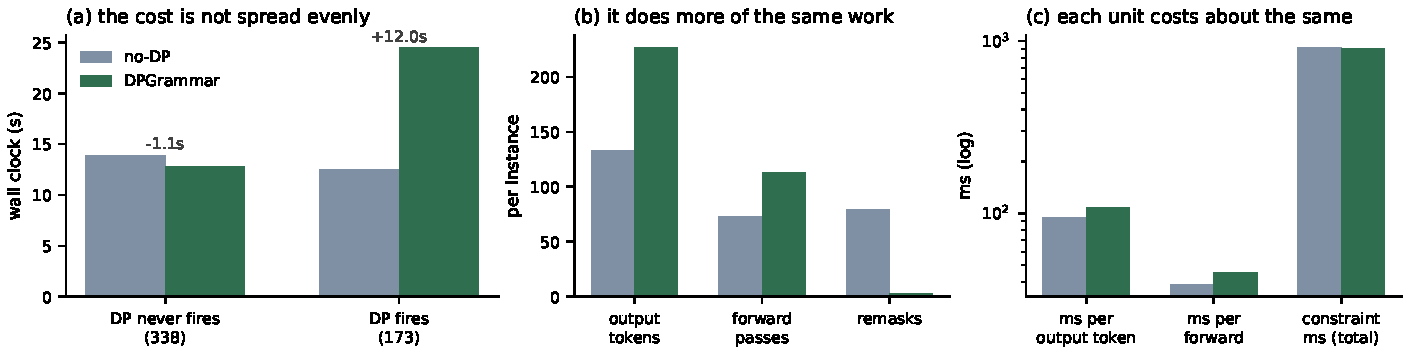
\includegraphics[width=\linewidth]{workload.pdf}
\caption{Averages per instance on JSONSchemaBench \texttt{medium}, split by
whether the repair layer ever fired. (a) The mean difference is concentrated in
the $173$ instances where it did; on the other $338$ the layer is slightly
faster. (b) On those instances it emits $71\%$ more tokens and needs
proportionally more forward passes, while remasking $28\times$ less. (c) Per
unit the two arms are close, and the constraint machinery costs the same in
both.}
\label{fig:workload}
\end{figure}

The bottleneck is not the search. The constraint machinery costs $909$\,ms
against the baseline's $920$, and grammar checks $22.5$\,ms against $11.2$. What
changes is how much gets written: the baseline stalls, remasking $79$ times and
stopping at $133$ tokens, while DPGrammar repairs and continues to $227$. That
takes $1.5\times$ the forward passes, each $1.2\times$ slower on the longer
sequence, which is the whole of the difference.

\section{Why validity alone is not enough}
\label{app:example}

Schema validity can be blind to a difference that matters, which is why
\S\ref{sec:metric} pairs it with a content floor rather than reporting it alone.
On \texttt{o78738} the schema asks for a course catalogue entry. Both arms
validate, so schema@1 scores them identically; what separates them is that the
unrepaired baseline stalls inside \texttt{prereqs}, emits two hundred lines of
whitespace, and closes the array empty:

\begin{center}
\footnotesize
\begin{minipage}{0.86\linewidth}
\begin{verbatim}
no-DP: valid, 4 populated leaves
[ { "code": "MATH 1001", "name": "Calculus I", "credits": "4",
    "description": "An introduction to calculus",
    "requirements": { "prereqs": [
                                       <200 lines of whitespace>
                      ], "coreqs": [] } } ]
\end{verbatim}
\end{minipage}
\end{center}

\noindent
DPGrammar reaches the same violation at position $120$, solves a three-position
span in which the parser admits fewer than two tokens on average, and the
decoder continues through the rest of the record:

\begin{center}
\footnotesize
\begin{minipage}{0.86\linewidth}
\begin{verbatim}
DPGrammar: valid, 12 populated leaves
[ { "code": "MATH 1001", "name": "Calculus I", "credits": "4",
    "description": "An introduction to calculus",
    "requirements": {
        "prereqs": [["MATH 0001", "MATH 0002"]],
        "coreqs":  [["MATH 1001", "MATH 1002"]] },
    "lectureHours": "3", "tutorialHours": "-", "labHours": "2",
    "note": "Recommended for first-year students" } ]
\end{verbatim}
\end{minipage}
\end{center}

\noindent
Neither output is wrong about the course; the baseline simply stops saying
anything, and validity cannot see the difference. Only the content floor
separates them, and it does so by $8$ populated leaves.

Neither instance is exceptional: across \texttt{medium}, $18.8\%$ of the
baseline's valid outputs carry fewer than five scalar leaves, against $12.1\%$
of ours.
